\section{Data and methodology}
\label{sec:method}

A carrier from an accelerating transmitter drifts in sky frequency, and over
a long track its power spreads across many channels. The analysis therefore
\emph{de-drifts} the data, shifting each integration's spectrum to follow a
trial drift rate before adding the integrations together.

\subsection{The de-drifted search statistic}
\label{sec:statistic}

The search statistic is the largest stacked signal-to-noise ratio anywhere on
the channel$\times$drift grid of a window's dynamic spectrum,
%
\begin{equation}
T(\mathbf{x})=\max_{\dot\nu,\;\nu}\;
\frac{\sum_{t} I\!\left(\mathbf{x},t,\nu+\dot\nu t\right)
       \big/\sigma^{2}(t,\nu+\dot\nu t)}
     {\left[\sum_{t}1\big/\sigma^{2}(t,\nu+\dot\nu t)\right]^{1/2}},
\label{eq:tstar}
\end{equation}
%
where $I(\mathbf{x},t,\nu)$ is the spectrum at sky position $\mathbf{x}$ in
integration $t$ and channel $\nu$, $\dot\nu$ is the trial drift rate, and
$\sigma(t,\nu)$ is the noise scale, both evaluated at the channel the track
occupies in that integration. $T_\star$ denotes the value at the star. The
time $t$ runs from the first integration, so the frequency that labels a track
is the one a carrier would occupy at the start of the block; a repeat epoch is
read at the cell the same convention fixes (\S\ref{sec:etacrv}).

Equation~\ref{eq:tstar} is the matched filter, and $T$ an absolute
signal-to-noise ratio, only if the noise is independent between integrations
and channels, which the analysis does not assume. The trigger is instead set
against the distribution $T$ takes in the data, measured in every window at
\NCtrl{} control positions on the same visibilities and through the same
stack. A value of $T$ is converted into a power by injected carriers recovered
through the unchanged pipeline (\S\ref{sec:pninetysel}). The controls lie,
from a fixed seed, in an annulus set by each block's synthesised and primary
beams. The noise scale $\sigma$ is their median absolute deviation at each
integration and channel, scaled to a Gaussian-equivalent standard deviation,
and the statistic is evaluated identically at the star and at each control.
The field read over is the whole primary beam: every \texttt{FIELD} entry in
which the star's primary-beam response reaches \BgFieldMinResp.

Spectra are extracted at the star's apparent position, never from images: for
each integration and native channel the pipeline forms the weighted vector
average of the phase-shifted visibilities in total intensity,
$I=(XX+YY)/2$. That is the dirty-map value at the star, an amplitude and not a
deconvolved flux density, so it is not a point-source measurement where the
field holds extended emission. The correction for the star's offset from the
phase centre is measured with injected carriers (Appendix~\ref{app:pbresp}).
Positions are propagated to the observation epoch for proper motion only; the
annual parallax and orbital motion are corrected window by window in
\S\ref{sec:pninetysel} and bounded for every component of a multiple in
Appendix~\ref{app:pbresp}. On-source time is counted per integration from the
delivered exposure records.
%
% FLAGS SENTENCE (v4.29 re-calibration fold; every number from reflagdecl_r29.py, round 2900)
The data are the archive's deliveries, recalibrated with ALMA's final flags
(and, for the \RflNEbLegacyWord{} blocks calibrated by legacy scripts, its online
flags and flux scaling) wherever a block sets a quoted limit or holds a
crossing: \RflNEbCore{} of the \RflNEbCoreAll{} such blocks, with
\RflNEbExtra{} more that hold repeat epochs or runner-up windows. The other
\RflNEbNot{} keep the delivered calibration: \RflNotClause; \RflNNotLim{} of
them set a quoted limit and
\RflNNotCross{} hold a crossing. On the \RflChNWin{} recalibrated Class~A
windows the rate at which control positions exceed the trigger changes by a
factor \RflChRatio{} (95 per cent interval \RflChLo--\RflChHi), which bounds the
chance expectation of the mixed calibration at \RflCeLo--\RflCeHi.
%
Every delivered channel is searched, without regridding, deconvolution or
edge trimming. A per-integration median along frequency removes the
continuum, and none is taken along time, so no feature narrow against the band
can be removed. Because the delivered channels are smoothed, a correction
computed from the correlator's own channel shape turns flux density times
channel width into a radiated power (Appendix~\ref{app:conventions}).

The search runs on the topocentric sky frequencies ALMA delivered, and every
drift rate quoted is the apparent one at the telescope. Two steps need the
star's own frame: comparing a crossing with the line catalogue, and reading a
repeat epoch at the \emph{predicted cell}, the single channel and drift rate
where the discovery's own fit puts a carrier. Both correct each block's
frequency axis for the Earth's motion and then for the star's systemic
velocity. That is the SIMBAD radial velocity \citep{SIMBAD2000}, queried on
\SimbadQueryDate, or zero where none exists -- \FrZeroVsysClause{}
(\S\ref{sec:sample}). Toward $\beta$~Pic the value of the ALMA CO analysis of
its disc is adopted.\footnote{\BpRecVsys\,km\,s$^{-1}$ \citep{Matra2017},
which this survey's own blocks reproduce; it exceeds the catalogued value by
about the template-mismatch offset the \textit{Gaia} pipeline documents for
stars this hot \citep{Blomme2023}.}

Two power quantities are defined in Table~\ref{tab:quantities}. The trigger
level $P_{\rm trig} = 4\pi d^{2}S\,\Delta\nu$ is the power at distance $d$ of a
carrier that makes $T_\star$ reach $T_{\rm trig}=\StageNullTrig$ in one native
channel of width $\Delta\nu$. The sensitivity $\mathrm{EIRP}_{90}$ is
calibrated by injecting synthetic carriers of known amplitude into the
calibrated visibilities of \SensNInj{} windows and recovering them through the
unmodified pipeline, one class factor being applied to every window. It is
nominal in that it excludes atmospheric decorrelation, so it is not a fully
calibrated completeness for a real carrier in every system
(\S\ref{sec:pninetysel}). Every limit quoted is the $\mathrm{EIRP}_{90}$ of its
own window, beside its native channel width, except the labelled
bare-threshold comparisons of \S\ref{sec:intro}; its error budget is
Table~\ref{tab:p90budget}. The amplitude scale is checked twice. An
independent reduction of the same AU~Mic visibilities is reproduced to
\PxJanRatio\,$\pm$\,\PxJanRatioErr, which tests the extraction and not ALMA's
flux transfer. The quiescent flux density of $\epsilon$~Eridani
\citep{Burton2022} is recovered to \PxEpsRatio\,$\pm$\,\PxEpsRatioErr, which
measures the scale to \SbEpsPct{} per cent. The absolute scale is therefore
carried at ALMA's own accuracy specification: $\pm\BudComb$ per cent for the
sample and $\pm\BudCombWorst$ for the \BudNHiWin{} Class~A windows in
\BudHiBandWord~\BudHiBands{} (\BudHiGHzList\,GHz).

The drift range is bounded by an acceleration, not by a frequency. Drift rate
and line-of-sight acceleration are one quantity in two sets of units,
%
\begin{equation}
\frac{\dot\nu}{\nu}=\frac{a_{\rm los}}{c}
\qquad\text{and so}\qquad
a_{\rm los}=\frac{c\,\dot\nu}{\nu},
\label{eq:accel}
\end{equation}
%
so a ceiling on $\dot\nu/\nu$ is the same physical limit in every band. The
default ceiling, \DriftCeilLo--\DriftCeilHi\,Hz\,s$^{-1}$\,GHz$^{-1}$, is the
acceleration of a transmitter orbiting a solar-type star at a few hundredths
of an au. That is the \citet{Mason2025} fiducial with a threefold margin, and
\AccelSheikhPct{} per cent of the \AccelSheikhNHz\,nHz that \citet{Sheikh2019}
recommend for a general search. It is widened for a planet host whose
innermost known planet demands more: as an acceleration it is
\AccelCeilMed\,m\,s$^{-2}$, the median over the Class~A windows, rising to
\AccelCeilMax\,m\,s$^{-2}$ on the \AccelNWide{} \AccelWideStar{} windows
(Fig.~\ref{fig:accel}). The grid is uniform in $\dot\nu$ and runs from the
negative ceiling to the first trial at or beyond the positive one
(Appendix~\ref{sec:edge}); it is fine enough that a carrier midway between two
trials loses no more than \DriftGridFineHalf{} of a native channel over the
longest track.
\textbf{The survey does not constrain a transmitter whose apparent
acceleration exceeds that range}: a carrier chirped faster (a chirp is not
distinguished from acceleration), one not bound to a known planet, or one whose
orbital and rotational accelerations together exceed it. The rotation of
$\beta$~Pictoris~b, around a star searched here and the fastest measured for a
planetary-mass object, alone corresponds to \AccelBpicRotNHz\,nHz
\citep{Sheikh2019}, above the ceiling. For transiting
TRAPPIST-1~b, the most demanding known case, \TrapPhaseHi{} per cent of the
orbital phase lies above the default ceiling. The widened grid used on its
star matches its maximum acceleration to within the $\pm\TrpAmaxPct$ per cent
its host's mass and orbit are known to, so between nothing and a sixth of the
phase lies above that grid.

\begin{figure}
\centering
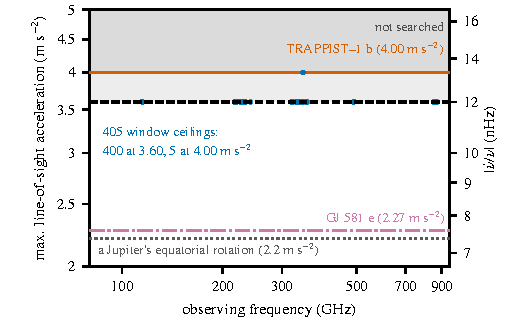
\includegraphics[width=\columnwidth]{figures/drift_acceleration.pdf}
\caption{What the drift search reaches, as a physical selection function: the
drift ceiling of each of the \NWinA{} Class~A windows (points), by
Equation~\ref{eq:accel}, against observing frequency, with the unsearched
region shaded and the same quantity as a fractional drift rate on the right.
Horizontal lines are the reference accelerations of \S\ref{sec:statistic}.}
\label{fig:accel}
\end{figure}

A drift search needs the maximum searched drift to cross of order one channel
over the on-source track, $\eta_{\rm drift} = |\dot\nu_{\max}|\tau_{\rm
track}/\Delta\nu_{\rm ch} \gtrsim 1$. \EtaDriftAOk{} of the \NWinA{} Class~A
windows satisfy it; the other \EtaDriftALo{} fall below because their tracks
are short, not because their channels are coarse. \EtaDriftBHi{} of the
\NWinB{} coarse windows also satisfy it but stay in Class~B, since crossing a
channel is necessary for drift discrimination and not sufficient
(Table~\ref{tab:quantities}); none of them holds a crossing. The per-window
catalogue carries $\eta_{\rm drift}$ for every window.

\subsection{From a crossing to a confirmed signal}
\label{sec:summary}

Every window passes through three steps in the same order -- the trigger, the
line attribution and the recurrence test -- which yield a \emph{crossing}, an
\emph{unattributed crossing} and, had one survived, a \emph{confirmed signal},
each defined in Table~\ref{tab:quantities}. None of the three is a
significance test. Every count below is read from the ledger of every crossing
the search produced, and is of primary crossings, one to a window.

\emph{The trigger.} The level on $T_\star$ carries no tail probability. $T$ is
not shown to follow any standard distribution under the null, and a window
holds between \TuCellsLo{} and $\TuCellsHi$ channel$\times$drift cells, so one
level buys very different protection in different windows. Every cell that
reaches it is recorded, not only the largest, because a carrier is masked as
effectively by a noise excursion as by a line.

\emph{The background.} A fixed threshold is not a fixed false-alarm rate, so
the number of crossings expected by chance is computed window by window from
the exceedance rate at that window's own control positions. That assumes a
star behaves like a control position in its own field, which the reserved
hold-out blocks test (\S\ref{sec:trigunif}). It also needs each block's
control ensemble to behave like noise, and one block, \BqFailBlock{} toward
\BqFailStar, fails that criterion (Appendix~\ref{sec:blockquality}). With
ALMA's final flags restored it holds no crossing, so the results are identical
with it and without it. The census's quality-passing data hold \CsNCrossQp{} crossings, all
of them Class~A, and these are the baseline every expectation is set against.
Of these, \BkFlagNCrossOther{} lies in a window the same diagnostic flags inside
a passing block; it is counted but withheld from the amplitude-dependent
tests. The \CeNTailCrossWord{} in archival-tail blocks enter no expectation
(Appendix~\ref{app:falsealarm}).

Two diagnostics say which crossing deserves attention first; neither decides a
disposition or is charged to the sensitivity. The first ranks $T_\star$
against the window's \NCtrl{} control positions, its lowest value,
$1/(\NCtrl+1)$, meaning that the star beat every control. It is a ranking
filter and not a significance test, because star and controls are not
demonstrably exchangeable. The annulus responds to whatever it surrounds, so
genuine CO toward $\beta$~Pictoris ranks below a control ring lifted by the
resolved disc (Appendix~\ref{app:radius}). Weighted star by star, the census
median rank is \BkRankBalSurv{} (\BkRankBalSurvLo--\BkRankBalSurvHi) and the
reserved blocks' \BkRankBalHo{} (\BkRankBalHoLo--\BkRankBalHoHi), both
consistent with the one half exchangeability implies. The second diagnostic, a
visibility-domain fit, asks whether the emission is at the stellar
coordinates, but at the trigger a noise maximum at the star also fits as a
point source there (\S\ref{sec:vistest}).

\emph{The line attribution} is a single database query, made on \MkListDate{}
and repeatable as it stands. A crossing within $\pm\MaskHalfKms$\,km\,s$^{-1}$
of a catalogued transition in the star's rest frame is \emph{attributed}. One
rule selects the species: covered by these setups and detected in discs or
molecular clouds, whatever a window was tuned to
(Appendix~\ref{app:linemask}). The half-width follows the Keplerian
line-of-sight velocities of gas surviving beyond a few au, with margin for the
systemic velocity. Halving it gives \FrAttrWTwentyFive{} attributed and
\FrUnattrWTwentyFive{} unattributed crossings at $\pm25$\,km\,s$^{-1}$,
against \FrAttrWFifty{} and \FrUnattrWFifty{} at
$\pm\MaskHalfKms$\,km\,s$^{-1}$. A coincidence is a statement about a
catalogue, not a property of a frequency, so an attribution is not a disposal:
all \CnCross{} crossings go on to the recurrence test whichever side of the
mask they fall. The price of the mask is that the survey constrains nothing
inside it.

\emph{The recurrence test.} A repeat counts only from a \emph{separated}
block, of another observing session and more than \EpSep{} day away, because
blocks of one session share calibrators, atmosphere, correlator setup and
interference. The day alone would not do: \QfNPairDrop{}
pairs of blocks here are of one session yet more than a day apart, the widest
by \QfSameSessMaxD\,d. Two readings are made. The \emph{line-recurrence check}
reads the one cell the discovery predicts in the star's frame, $\pm\RqDvLo$ to
$\pm\RqDvHi$\,km\,s$^{-1}$ wide. It recovers an emitter at rest in that frame,
as a line is, and a null there bounds only such an emitter, never a drifting
or re-tuned carrier. The \emph{trajectory comparison} asks whether one bounded
trajectory inside the drift grid joins two crossings. It can reject an
association between them but cannot accept one, and it cannot establish an
artificial origin for either. Table~\ref{tab:quantities} defines what a
confirmation needs; only part of the sample has a separated block at all
(\S\ref{sec:mmdifferent}).

The chain is shown to find what it is meant to find by the injected carriers
of \S\ref{sec:pninetysel} and by $\beta$~Pictoris CO, a real feature at a
known stellar position, recovered and localised in two transitions and
\CsBpCoBlocks{} execution blocks (\S\ref{sec:bpicval}).


\begin{table*}
\centering
\caption{The quantities and the three words this paper uses, defined once.
Every term below is used in this sense throughout and in no other. The
distinction the first three rows draw is the one the limits of
\S\ref{sec:pninetysel} turn on: a crossing is a single-epoch event, and a
confirmed signal needs a second and separated epoch that no sensitivity
supplies.}
\label{tab:quantities}
\small
\begin{tabular}{@{}p{0.145\textwidth}p{0.825\textwidth}@{}}
\hline
Term & Definition \\
\hline
Crossing &
A channel\,$\times$\,drift cell at the stellar position reaching
$T_\star\geq\StageNullTrig$ in one execution block; neighbouring channels
above the trigger belong to one crossing. The largest in a window is its
\emph{primary} crossing and any other a \emph{secondary} one, and because the
largest cell is the window's own statistic a secondary crossing exists only
where a primary one does. An event requiring investigation; no claimed
significance. \\
Unattributed crossing &
A crossing lying more than $\MaskHalfKms$\,km\,s$^{-1}$ in the star's frame
from every transition of the line catalogue. That is a reproducible frequency
coincidence; which coincidences are astrophysically plausible is a separate
judgement, stated with each one. A target for follow-up; not a detection. \\
Confirmed signal &
The same carrier found again in a \emph{separated} block -- a different
observing session, more than \EpSep{} day from the discovery -- in one of two
ways: recovered at the cell the discovery predicts in the star's frame (the
\emph{line-recurrence check}), or seen in three or more separated epochs that
one orbit fits, the third where the other two predict it. The check recovers
only an emitter at rest in the star's frame, as a line is, so a null there
never excludes a drifting or re-tuned carrier. A pair of crossings that one
bounded trajectory joins is \emph{open}, not confirmed: the window searched,
$\pm\WdHalfKms$\,km\,s$^{-1}$, is wider than the $\pm\EcVexcKms$\,km\,s$^{-1}$ an
orbit at the drift ceiling can produce, so the joining test can reject a pair and
cannot accept one (Table~\ref{tab:pairs}). For \ZcNoRepSys{} Class~A systems
the archive holds no separated block at the frequency, so no sensitivity makes
a confirmed signal possible there. \\
$P_{\rm trig}$ &
The power of a carrier that makes $T_\star$ reach the trigger in one native
channel. An internal pipeline level: not a sensitivity, not a
significance. \\
$\mathrm{EIRP}_{90}$ &
The power at which nine injected carriers in ten produce a crossing at the
star: a measured single-epoch trigger completeness, not a detection
probability. Calibrated by injection in \SensNInj{} windows, one class factor
applied to every window; each injected window's own point
($\times\SensIndivFacLo$--$\times\SensIndivFacHi$) is in the data archive.
The factor is interpolated within the injected configurations for
\NgNInterpWin{} windows and extrapolated beyond them for \NgNExtrapWin{}
(\S\ref{sec:pninetysel}).
Nominal in one respect: it excludes atmospheric decorrelation, which
Table~\ref{tab:persys} gives system by system. \\
Class~A &
The primary experiment, defined by channel width: \NWinA{} fine-channel
windows, median \ChanAMedKHz\,kHz, toward \NSysA{} systems over
\UnionClassA\,GHz of union bandwidth, \EtaDriftAOk{} of which satisfy
$\eta_{\rm drift}\gtrsim1$ (\S\ref{sec:statistic}). \\
Class~B &
The secondary experiment: \NWinB{} coarse-channel windows, mode
\ChanBModeMHz\,MHz, constraining a persistent unresolved excess. Never a
carrier search: in \ScCoarseNoDrift{} of them no searched drift leaves one
channel, and in the other \EtaDriftBHi{} the whole searched range moves a
carrier \ScBhEtaLo--\ScBhEtaHi{} channels, which registers one but does not
discriminate it (\S\ref{sec:statistic}). \\
The sample &
Neither volume-limited nor representative of the solar neighbourhood: the
stars ALMA happened to observe for other reasons (\S\ref{sec:sample}). \\
\hline
\end{tabular}
\end{table*}
